\documentclass{beamer}
\setbeamertemplate{navigation symbols}{}

\usepackage{beamerthemeshadow}
\usepackage{multirow}
\usepackage{rotating}
\usepackage[latin1]{inputenc}
\begin{document}
\title{Review on boosting methods}  
\author{Vu Tuan Hung and DO Quoc Khanh}
\institute{T�l�com ParisTech}
\date{\today}

\setbeamertemplate{caption}[numbered]
\beamertemplatetransparentcovered

\begin{frame}
\titlepage
\end{frame}

\begin{frame}\frametitle{Table of contents}\tableofcontents
\end{frame}

\section{Two-class problem}

\begin{frame}
    \frametitle{Common model}
    \begin{itemize}
        \item The goal: give a common model that can explain boosting algorithms, and that can help to construct other similar methods.
        \item View boosting as iterative algorithms of optimization in numerical/function space.
        \item Loss function $L(y, F)$.
        \item Choose $d_m$ direction of descent (gradient descent, steppest descent, Newton etc.)
        \item Look for $f_m \approx d_m$.
        \item $\mathcal{F} = \sum\limits_{m=1}^M \mathcal{Q}_m$.
    \end{itemize}
\end{frame}

\begin{frame}
    \frametitle{Summary}
    \begin{table}\centering
    \begin{tabular}{|c|c|c|c|}
        \hline
          & $L(y,F)$ & $d_m$/$\beta_m$ & pop-ver \\
         \hline
         Discrete AB & $e^{-yF}$ & steppest descent & No \\
         \hline
         Real AB & $e^{-yF}$ & direct optim & Yes \\
         \hline
         Gentle AB & $e^{-yF}$ & Newton step & Yes \\
         \hline
         LS Boost & $(y-F)^2$ & steppest descent & No \\
         \hline
         LAD TB & $\vert y - F\vert$ & grad/tree & No \\
         \hline
         M TB & Huber & grad/tree & No \\
         \hline
         Logit B & $\log(1+e^{2F}) - 2y^{*}F$ & Newton step & Yes \\
         \hline
         L2 TB & $\log(1+e^{-2yF})$ & grad/tree & No \\
         \hline
         Lk TB & - Binomial Likelihood & grad/tree & No \\
         \hline
    \end{tabular}
    \caption{Summary on boosting algorithms.}
    \label{sum_tab}
\end{table}
\end{frame}

\section{Multi-class problem}

\begin{frame}
    \frametitle{Traditional approach}
    \begin{itemize}
        \item $J$-class problem.
        \item Transformation of $y$ into $N\times J$-binary matrix.
        \item Divise the problem into $J$ binary problems.
        \item Two-class algorithms $\rightarrow F_j, j = 1:J$.
        \item Output for each $\textbf{x}$ : $arg\max\limits_{j=1:J} F_j(\textbf{x})$
    \end{itemize}
\end{frame}

\begin{frame}
    \frametitle{Traditional approach}
    \begin{figure}[ht]\centering
  	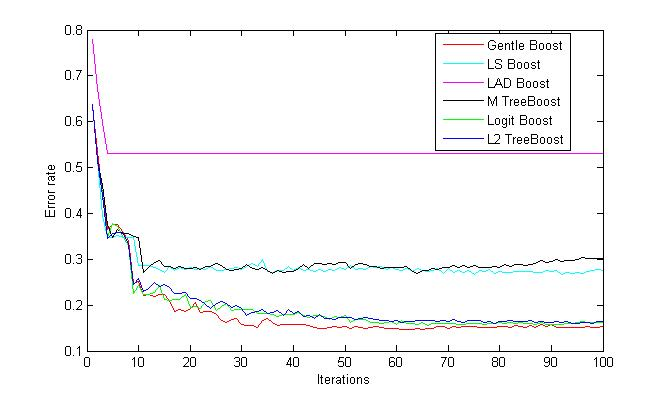
\includegraphics[width=0.7\textwidth]{comp_MH.jpg}
  	\caption{Comparison of the performances of \textsl{AdaBoost.MH} using $6$ two-class boosting methods, experiments on simulated data with $0 \%$ Bayes error.}
  	\label{comp_MH}
\end{figure}
\end{frame}

\begin{frame}
    \frametitle{Other generalizations}
    \begin{itemize}
        \item Logit Boost for $J$ classes and Lk TreeBoost.
        \item Can use our model for derivation.
    \end{itemize}
    \begin{figure}[ht]\centering
  	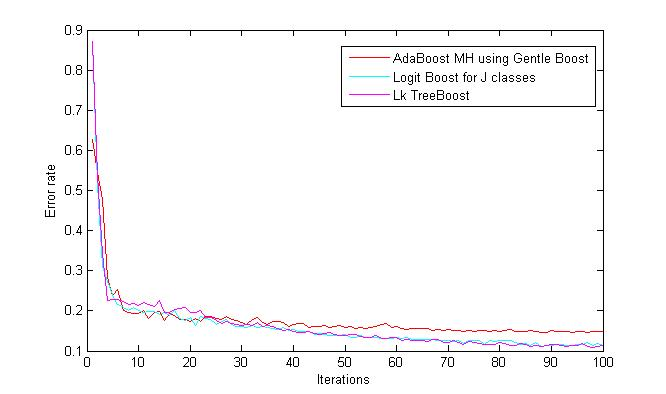
\includegraphics[width=0.7\textwidth]{multi_comp0.jpg}
  	\caption{Multi-class classification on simulated data, $J = 4$, Bayes error $0\%$.}
  	\label{multi_comp0}
\end{figure}
\end{frame}

\section{Experiments}

\begin{frame}
    \frametitle{Questions}
    \begin{center}
        ?
    \end{center}
\end{frame}

\end{document}